A peephole optimiser rewrites assembly code to make ik more efficient, in terms of processor cycles or memory usage. The general procedure is:
\begin{enumerate}
\item assembly parsing;
\item division in basic blocks;
\item optimisation;
\item assembly generation.
\end{enumerate}
See also figure~\ref{fig:diagram}. We discuss stages 1 and 4 first and then stage 2 and stage 3.

\subsection*{Assembly parsing and generation}
As an assembly program in the form of a set of text strings is difficult to process, the optimiser translates the input to an intermediate representation (ir) in the first stage. This translation is called \emph{parsing}. The resulting representation is a list of Python objects, where each object represents an assembly instruction. After optimising, the resulting intermediate representation is translated back to assembly code. Ideally, when no optimisation is done between parsing assembly and regenerating assembly, the composite function $4\circ 1$ is the identity function on the set of all assembly programs. (In our implementation, comments are left out in some cases, and spacing is sometimes changed.)

\subsection*{Division in basic blocks}
Before optimising, the ir is split in \emph{basic blocks}. A basic block is a set of consecutive instructions having a single entry point and a single exit point. By definition, only the first line $i_1$ of a basic block $(i_1, \ldots, i_k)$ can be a jump destination and only the last line $i_k$ can be a jump. Therefore, the execution flow is always $i_1\rightarrow i_2 \rightarrow \cdots \rightarrow i_k$. This property reduces the complexity of doing certain optimisations on instructions in a basic block.

Basic blocks can in turn be divided in functions, linked together by \emph{jump and link} instructions, \code{jal}. We call the set of instructions in a function a \emph{frame}. Frames have a single entry point (on frame level), but not necessarily a single exit point.

\subsection*{Optimisation}
In the optimisation stage, the original intermediate representation $A$ is transformed into a new ir $B$, such that
\begin{enumerate}
\item the new representation $B$ has the same \emph{meaning} as $A$, in terms of program output and behaviour;
\item the execution of the program corresponding to $B$ takes less processor cycles and uses less memory.
\end{enumerate}

Our optimiser performs serveral types of optimisations:
\begin{itemize}
\item Vul maar in.
\end{itemize}


\begin{figure}[H]
\centering
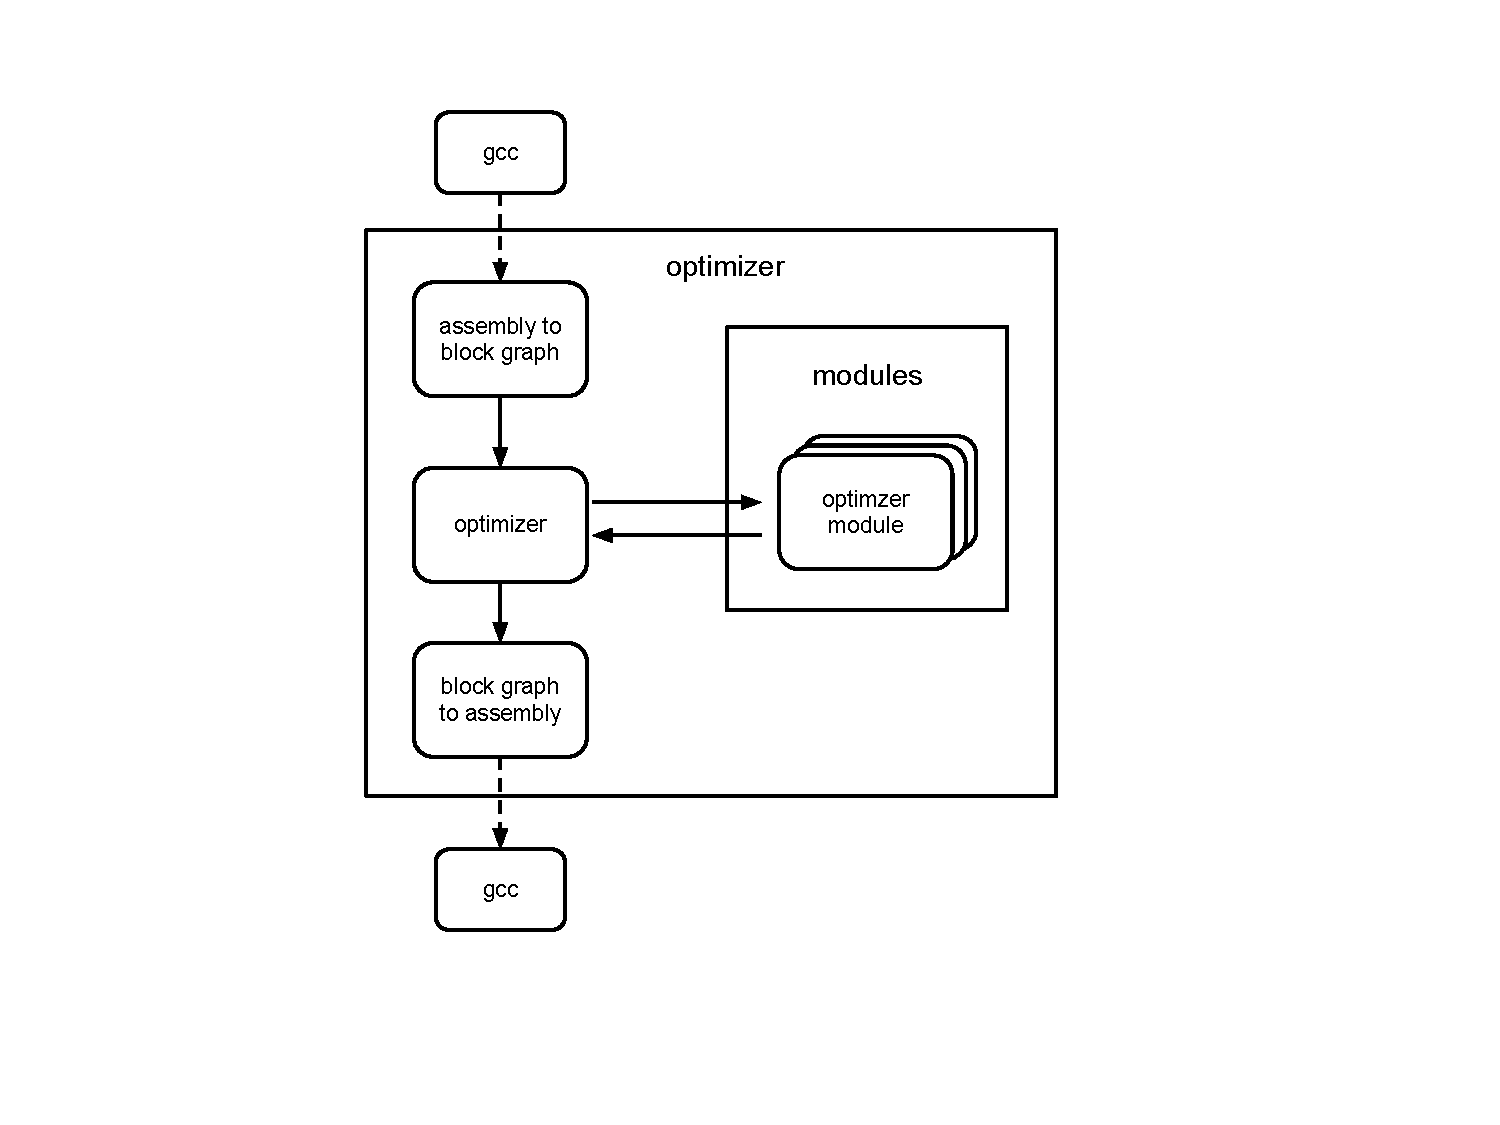
\includegraphics[viewport= 170 90 510 490, clip=true]{diagram}
\caption{Optimiser design diagram.}
\label{fig:diagram}
\end{figure}

